字符串 $S$ 的 SAM 是一个接受 $S$ 的所有后缀的最小 DFA 。例如 $S=\text{abbb}$ 的 SAM 如下:
\begin{figure}[H]
    \centering
    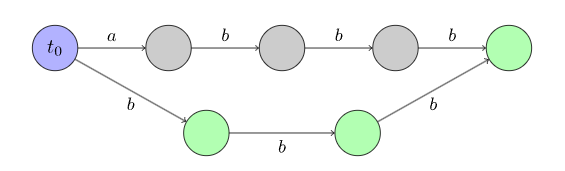
\includegraphics[width=0.45\textwidth]{src/string/SAM.png}
    \label{sam}
\end{figure}
SAM 的后缀链接构成了原串的后缀树。

对于代码实现,首先,我们实现一种存储一个转移的全部信息的数据结构。如果需要的话,你可以在这里加入一个终止标记,也可以是一些其它信息。我们将用一个 map 存储转移的列表,允许我们在总计 $O(n)$ 的空间复杂度和 $O(n\log |\Sigma|)$ 的时间复杂度内处理整个字符串。
\begin{minted}{cpp}
struct state {
    int len, link;
    std::map<char, int> next;
};
\end{minted}
SAM 本身将会存储在一个 \verb|state| 结构体数组中。我们记录当前自动机的大小 \verb|sz| 和变量 \verb|last| ,当前整个字符串对应的状态。
\begin{minted}{cpp}
const int MAXLEN = 100000;
state st[MAXLEN * 2];
int sz, last;
\end{minted}
我们定义一个函数来初始化 SAM(创建一个只有初始状态的 SAM)。
\begin{minted}{cpp}
void sam_init() {
    st[0].len = 0;
    st[0].link = -1;
    sz++;
    last = 0;
}
\end{minted}
最终我们给出主函数的实现:给当前行末增加一个字符,对应的在之前的基础上建造自动机。
\begin{minted}{cpp}
void sam_extend(char c) {
    int cur = sz++;
    st[cur].len = st[last].len + 1;
    int p = last;
    while (p != -1 && !st[p].next.count(c)) {
        st[p].next[c] = cur;
        p = st[p].link;
    }
    if (p == -1) {
        st[cur].link = 0;
    } else {
        int q = st[p].next[c];
        if (st[p].len + 1 == st[q].len) {
            st[cur].link = q;
        } else {
            int clone = sz++;
            st[clone].len = st[p].len + 1;
            st[clone].next = st[q].next;
            st[clone].link = st[q].link;
            while (p != -1 && st[p].next[c] == q) {
                st[p].next[c] = clone;
                p = st[p].link;
            }
            st[q].link = st[cur].link = clone;
        }
    }
    last = cur;
}
\end{minted}